\documentclass[letterpaper]{uafthesis}

\usepackage{ppl} % Bitches love the Paladino font.
\usepackage{amsmath, amssymb, amsfonts}
\usepackage{graphicx, float} % Graphics stuff
\usepackage{verbatim} % Mostly for the comment environment.
\usepackage{chapterbib} % The grad school likes bibliographies per-chapter.

\input custom-macros.tex

\includeonly{introduction, ch1, ch2}

\begin{document}

\title{The Measurement of Anisotropic Thermal Conductivity of Snow With Needle Probes}
\author{Joshua Holbrook}

\degreeyear{2011}
\degreemonth{May}
\degree{Master of Science}
\numberofmembers{3} % Make sure this is right! The grad school hates empty
                    % signature lines.
\prevdegrees{B.S.}
\college{College of Engineering and Mines}

\makesig
\maketitle

% Wondering when to use `input' and when to use `include?'
% read http://en.wikibooks.org/wiki/LaTeX/Basics#Big_Projects .
\begin{abstract}
  \input abstract.tex
\end{abstract}


%Table of Contents and such
\tableofcontents
\listoffigures
\listoftables
\listofothermaterials
\listofappendices

\begin{acknowledgements}
  \input acknowledgements.tex
\end{acknowledgements}

\begin{quotepage}
  \input quotepage.tex
\end{quotepage}

\chapter{Introduction}
\label{sec:introduction}
\bigskip

\section{Motivation}
\label{sec:introduction:motivation}

\marginpar{Expand on this? Cite research tackling this problem through other means?}

The thermal properties of snow are of interest to scientists studying Arctic and
sub-Arctic climates because, during the long, cold winters in this region,
snow's thermal behavior plays a critical role in determining the net energy
balance between Earth's surface and the atmosphere. After all, any heat transfer
occurring between the Earth and the atmosphere over snow-covered ground must go
through the snow first (Figure \ref{fig:climate}). In fact, the snow
itself may store and release energy over time.

\begin{figure}[h]
\centering
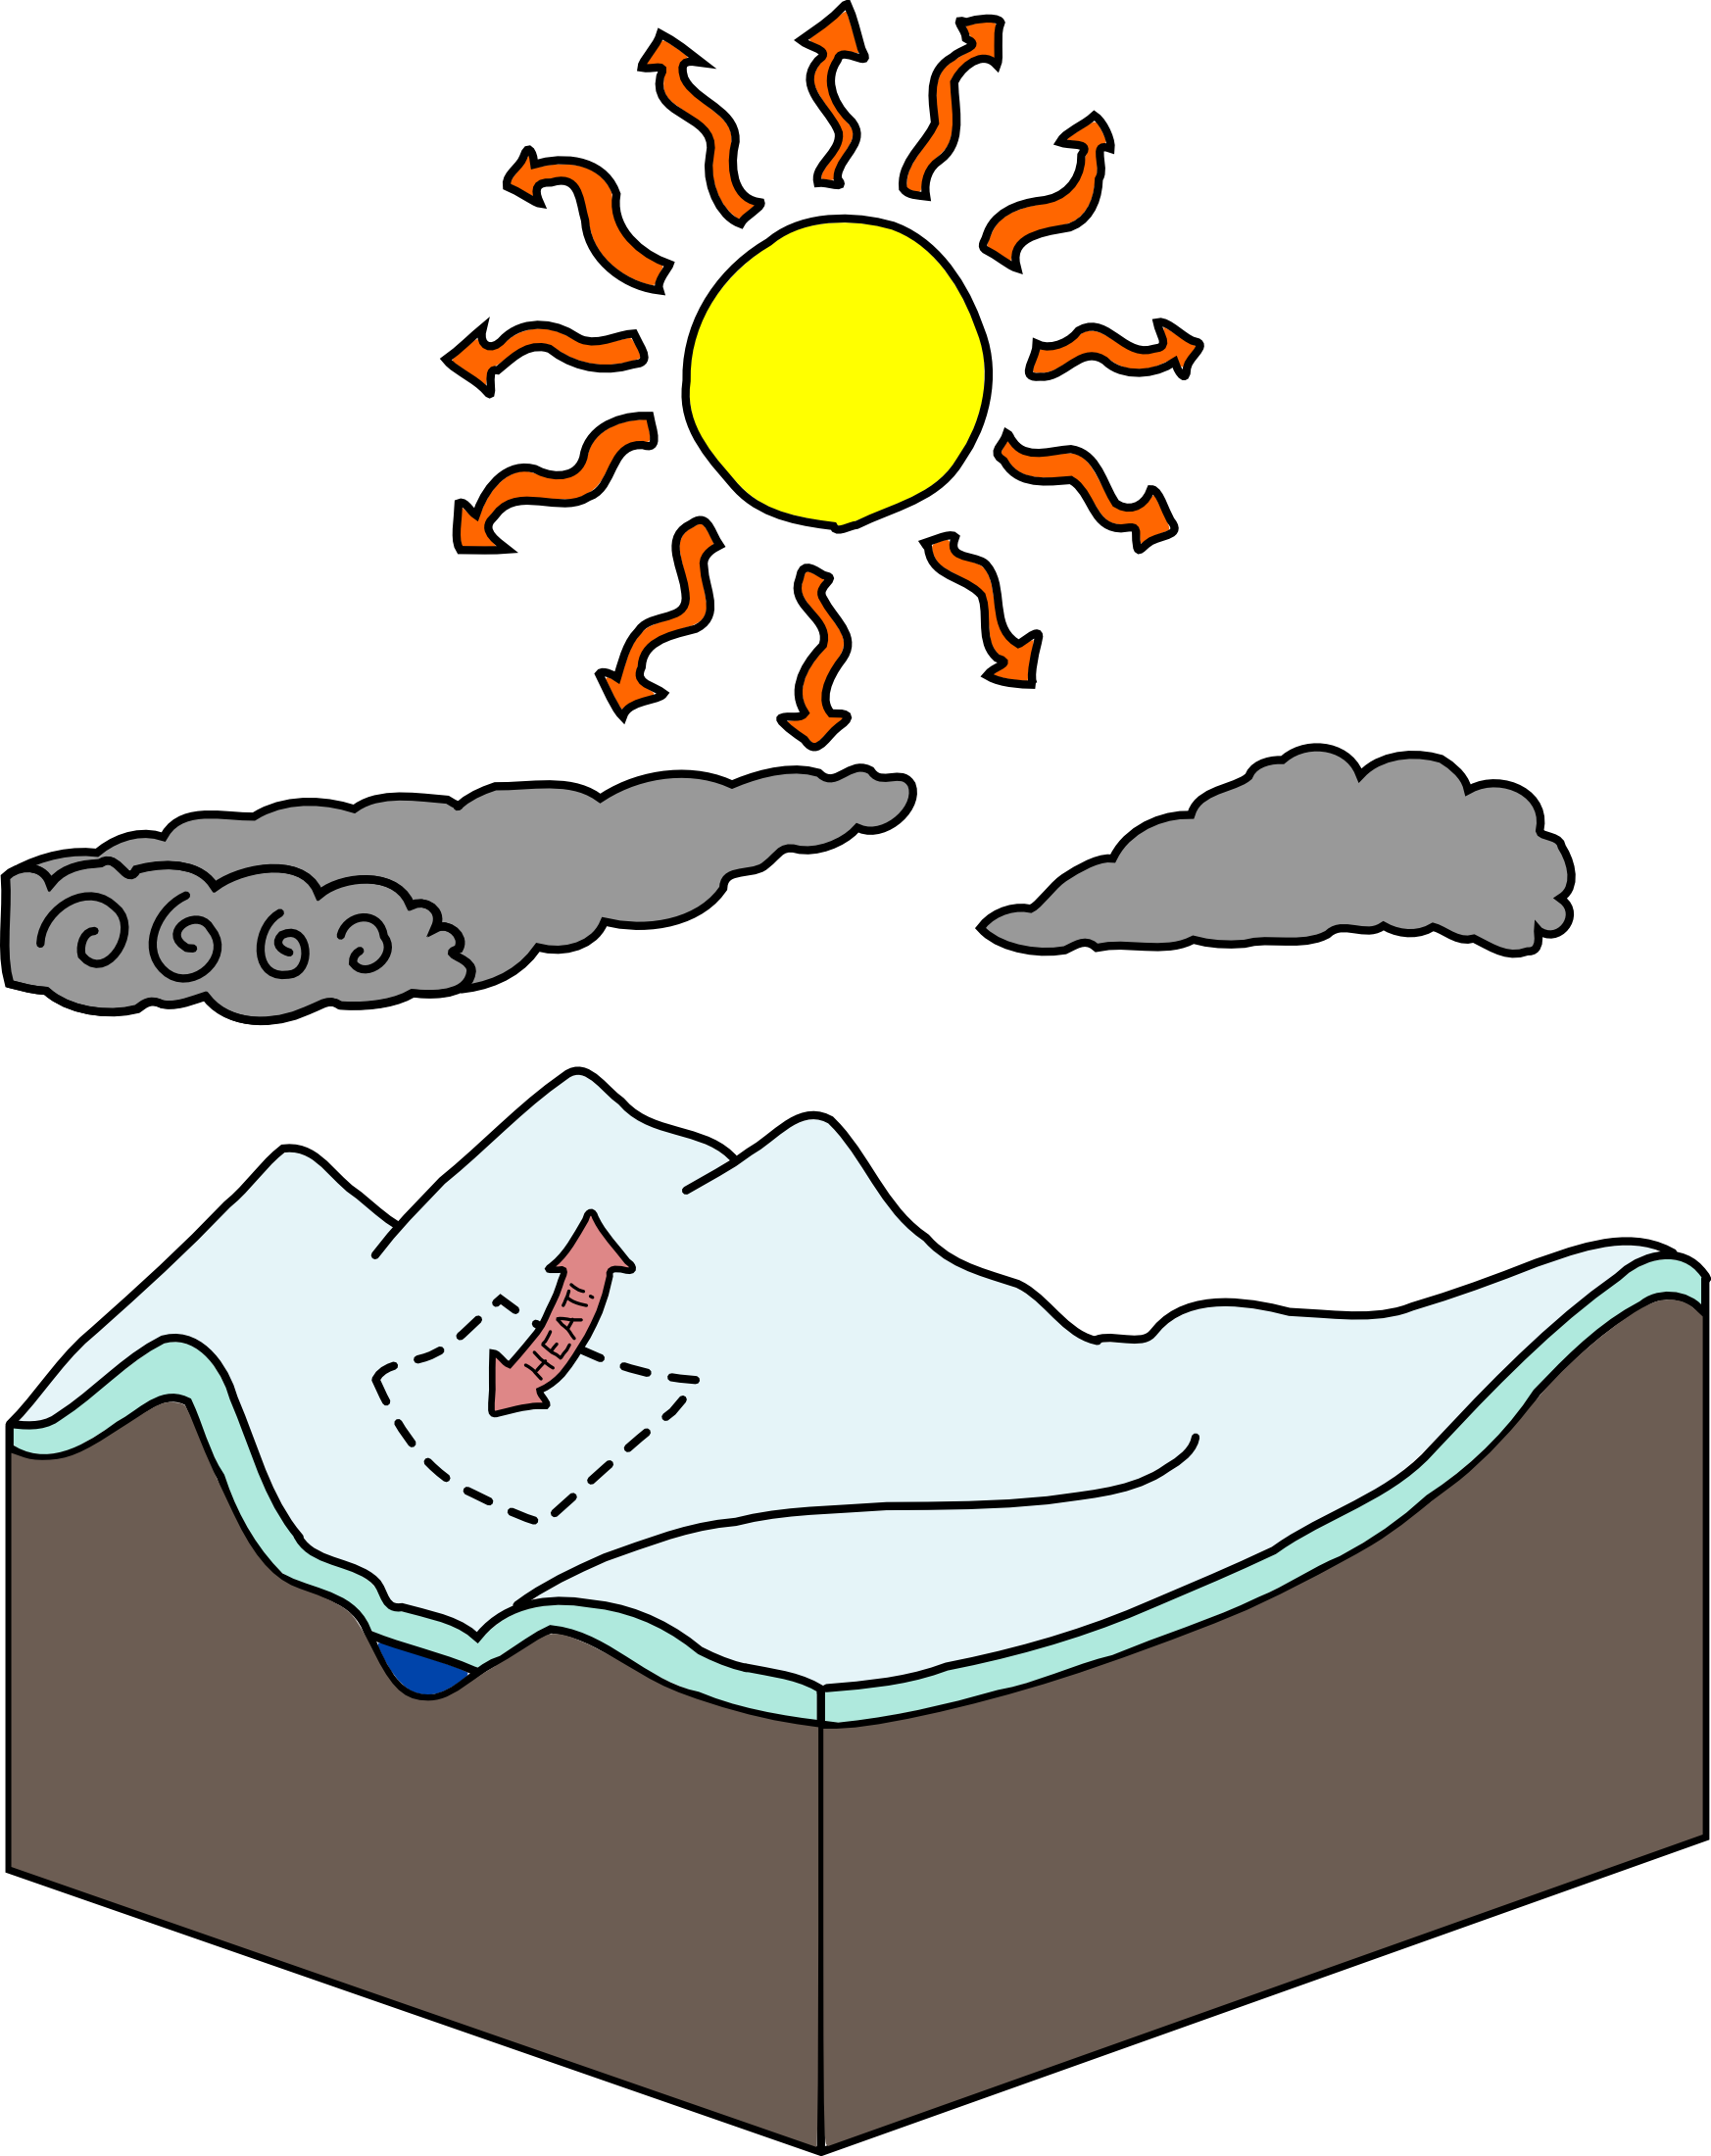
\includegraphics[width=0.4\textwidth]{fig/climate.png}
\label{fig:climate}
\caption{Arctic and Sub-Arctic climate is affected largely by heat transfer
between the atmosphere and the ground. Snowpack adds thermal resistance
transfer, affecting this heat transfer.}
\end{figure}

This energy transfer is critical in accurate climate models for these cold
regions, therefore the effective thermal conductivity of snow is a very
important factor for these models, and has been studied thoroughly \cite{sturm1, sturm2, sturm3}.


\section{Needle Probes: Basic Principles}
\label{sec:introduction:needles}

A more typical technique for measuring thermal conductivity, especially in the
context of engineering materials such as building insulation, is the guarded
hot plate. For this technique, a constant temperature gradient is induced across
the material, and heat flux over the material is measured.  By Fourier's Law,
\(k = \frac{\dot{q}l}{A\Delta T}\), where \(\dot{q}\) is the heat flux, \(A\) is
the cross-sectional area of the sample, \(l\) is the sample thickness, and 
\(\Delta T\) is the temperature difference across the sample. This technique
works great in many cases. However, it is difficult to take guarded hot plate
measurements of snow because it changes structure immediately after virtually
any physical interaction.

Another technique used for porous materials, such as soils and snow, is the
needle probe method. A needle probe consists of a long, thin needle with heating
wire running along its interior, and a temperature sensor in the center. This
configuration approximates an infinite line of constant-flux heat source
(Figure \ref{fig:needle_xsect}) \cite{basictheory}.

\begin{figure}[h]
\centering
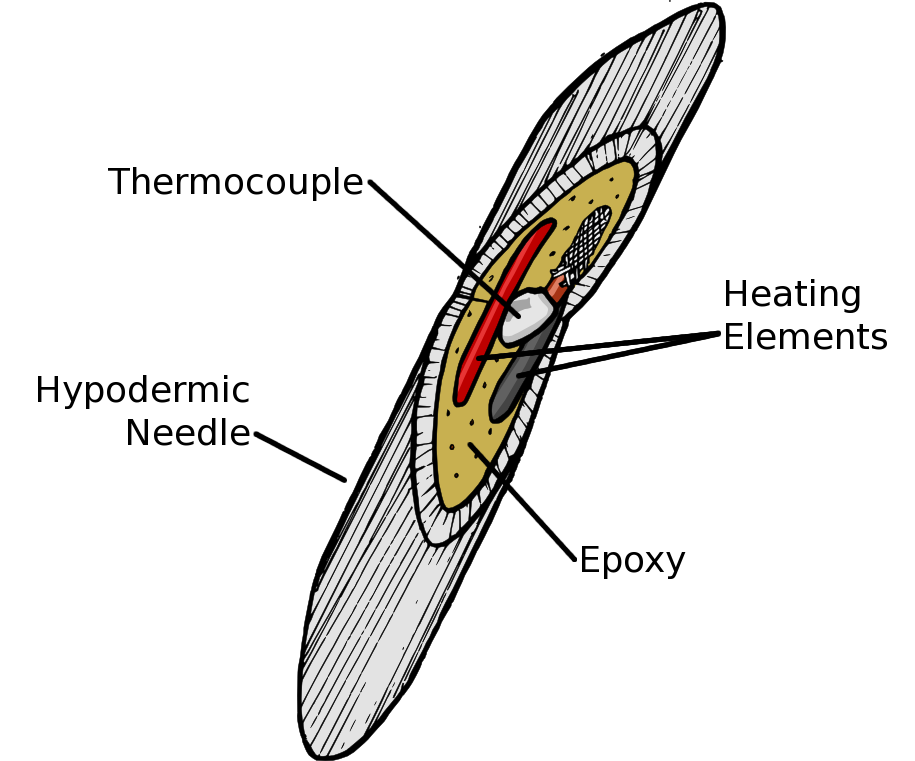
\includegraphics[width=0.2\textwidth]{fig/needle_xsect.png}
\label{fig:needle_xsect}
\caption{An illustration of a needle probe in cross-section. Note that the heat
trace in many needle probes, including the one used in experiments for this
research, actually wraps around an inner core instead of running axially through
the needle.}
\end{figure}

This needle is inserted into the material whose thermal conductivity is being
measured, and a constant voltage is applied to the needle's heating element.
This causes a constant heat flux along the needle, and, knowing the resistance
of the heat trace, this heat flux may be calculated. This causes the material's
temperature near the needle to rise (Figure \ref{fig:heating_curve}. After some
given amount of time, the heating element is turned off, and the temperature
around the needle begins to fall back towards ambient (Figure \ref{fig:cooling_curve}).
The temperature data measured over time for these two periods are called the
heating cooling curves, respectively.  Based on the slopes of these
curves as a function of \(\ln(t)\) and approximate analytical solutions for
these situations, effective thermal conductivity may be calculated.

In this document, studies concentrate on the heating curve. In fact, the
numerical and analytical approaches focus exclusively on the heating curve. This
is because the initial conditions of the cooling curve problem depend on the
final conditions of the heating curve problem, and because many references spend
more time describing the derivation of the heating curve and list the cooling
curve as being possible to derive ``from an analogous argument.'' However, the
benchtop and in-situ measurements use both heating and cooling curves.

\section{Difficulties with the Needle Probe Method}

It should be noted that the needle probe method is not without its caveats. For
instance, it was shown that convection can and will occur in natural snowpack
\cite{sturm3}. In addition to the fact that convection in snowpack can change the
entire assumed heat transfer dynamic, heating the needle itself can cause this
convection to occur. This means that, when measurements are taken, there will
not only be ``transient'' regions due to early-time behavior, but also regions
where convection becomes a major force. Practically, this means that linear
portions (with respect to \(\ln(t)\)) must be found in between these regions
of instability.

\section{Snow Metamorphic Principles}
\label{sec:introduction:metamorphic}

The structure of a snowpack is strongly influenced by outside environmental
factors. Immediately after falling from the sky, snow begins to metamporphose as
it compacts under its own weight. In addition to this, temperature gradients
cause snow to sublimate and re-form in different regions of the snowpack, in a
process called vapor transport. Vapor transport is best known for causing
depth hoar, but occurs throughout the snowpack. Other events, such as
freeze-thaw events, may also change the form of snow. All these metamorphic
processes on snow cause it to form regions of varying thermal conductivity. In
some cases, these regions may form sharp, distinct layers with constant
properties, while in other cases they have continuously varying properties.

\section{Anisotropic Aggregate Behavior in Snow}

At a macroscale, alternating regions of low-conductivity and high-conductivity
material may act in the aggregate as a single material of anisotropic thermal
conductivity---In other words, the effective thermal conductivity parallel to
the orientation of the layers may be different than the effective thermal
conductivity orthogonal to the layers.

For example, suppose a composite exists of alternating layers, each of thickness
\(l\) and with conductivities \(k_1\) and \(k_2\), as in Figure
\ref{fig:ex_laminate}:

\begin{figure}[h]
\centering
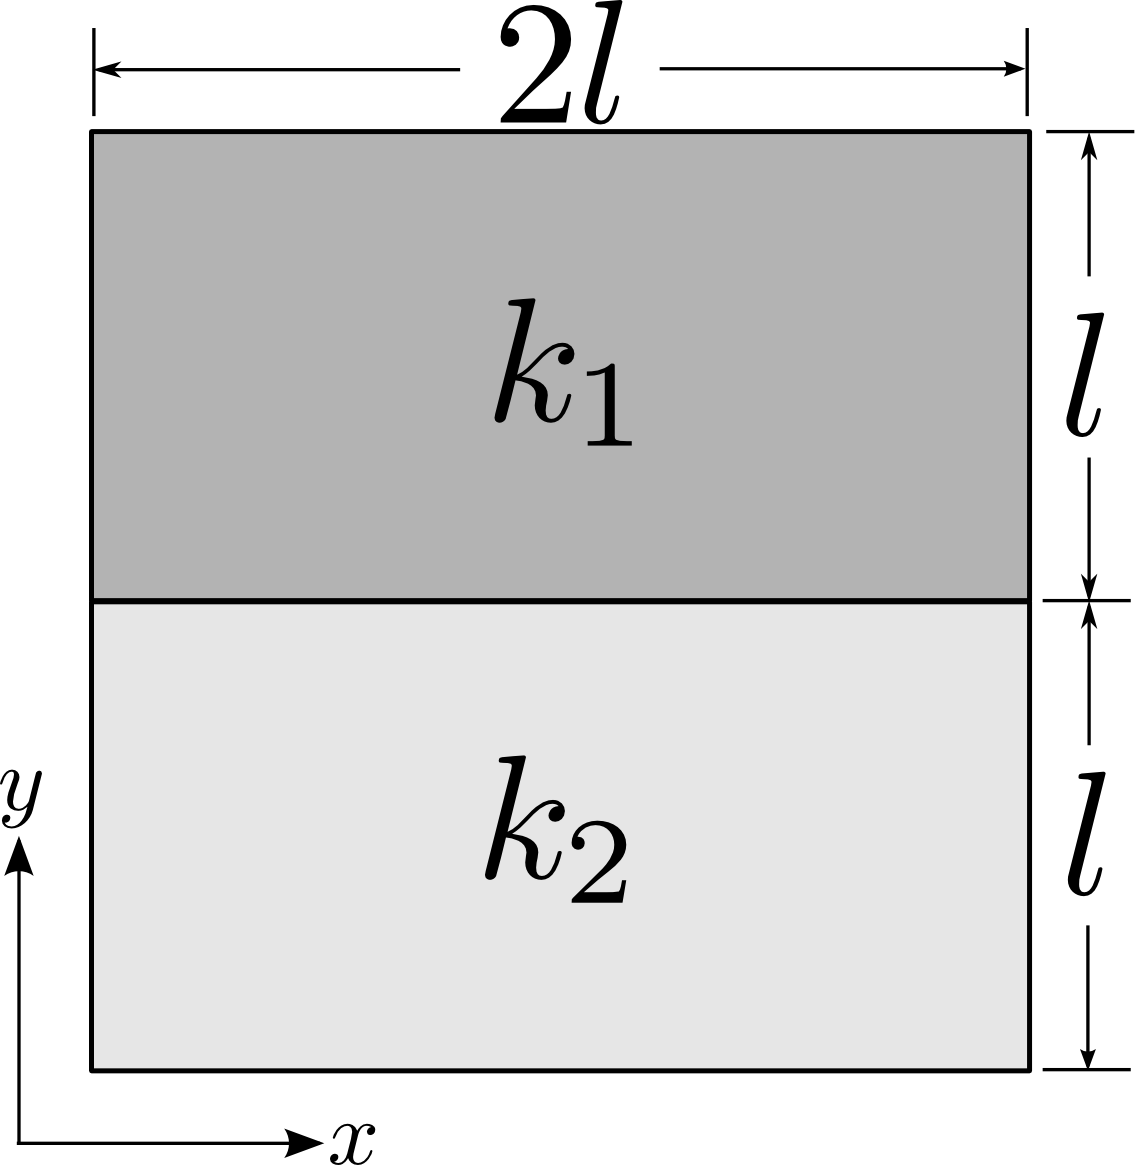
\includegraphics[width=0.3\textwidth]{fig/ex_laminate.png}
\label{fig:ex_laminate}
\caption{Two layers of materials create a different net conductivity value in the vertical direction than in the horizontal direction.}
\end{figure}

In the vertical direction, the effective thermal conductivity is
\(\frac12(k_1 + k_2)\). However, in the horizontal direction the effective
thermal conductivity is \(2\left( \frac1{k_1} + \frac1{k_2} \right)^{-1}\). An analogous analysis could be applied to a number of geometries.


\section{Measuring Anisotropic Thermal Conductivity}

This aggregate anisotropy brings a number of questions:

\begin{itemize}
\item Can anisotropic thermal conductivity in snow be measured with the needle
probe technique at all? If so, how accurately, and how many measurements would
one need?
\item How severe is anisotropy in snow? Is the amount of anisotropy
significant?
\item Is anisotropy in snow predictable? That is, could one take a single
measurement and extrapolate from it the anisotropic thermal conductivity?
\item Can anisotropy in snow explain historical differences between various
thermal conductivity measurements of snow using both the guarded hot plate and
needle probe techniques?
\end{itemize}

This document aims mostly to answer the first question. Developing a way
to measure anisotropic thermal conductivity with needle probes should enable
future researchers in answering the other questions. However, these other
questions will also, in part, be addressed.

\section{Anisotropic Model}

In every model studied, it has been assumed that the horizontal plane has the
same thermal conductivity and that only the vertical direction differs. In other
words, \(k_x = k_y = k_{xy} \ne k_z\). Each model aims to predict the measured
conductivity, \(k_{\textrm{meas}}\) as a function of angle.

In both analytical and numerical models and in the measurements, the angle
parameter, \(\theta\), is measured from the horizontal plane, as in Figure 
\ref{fig:angle}.

\begin{figure}[h]
\centering
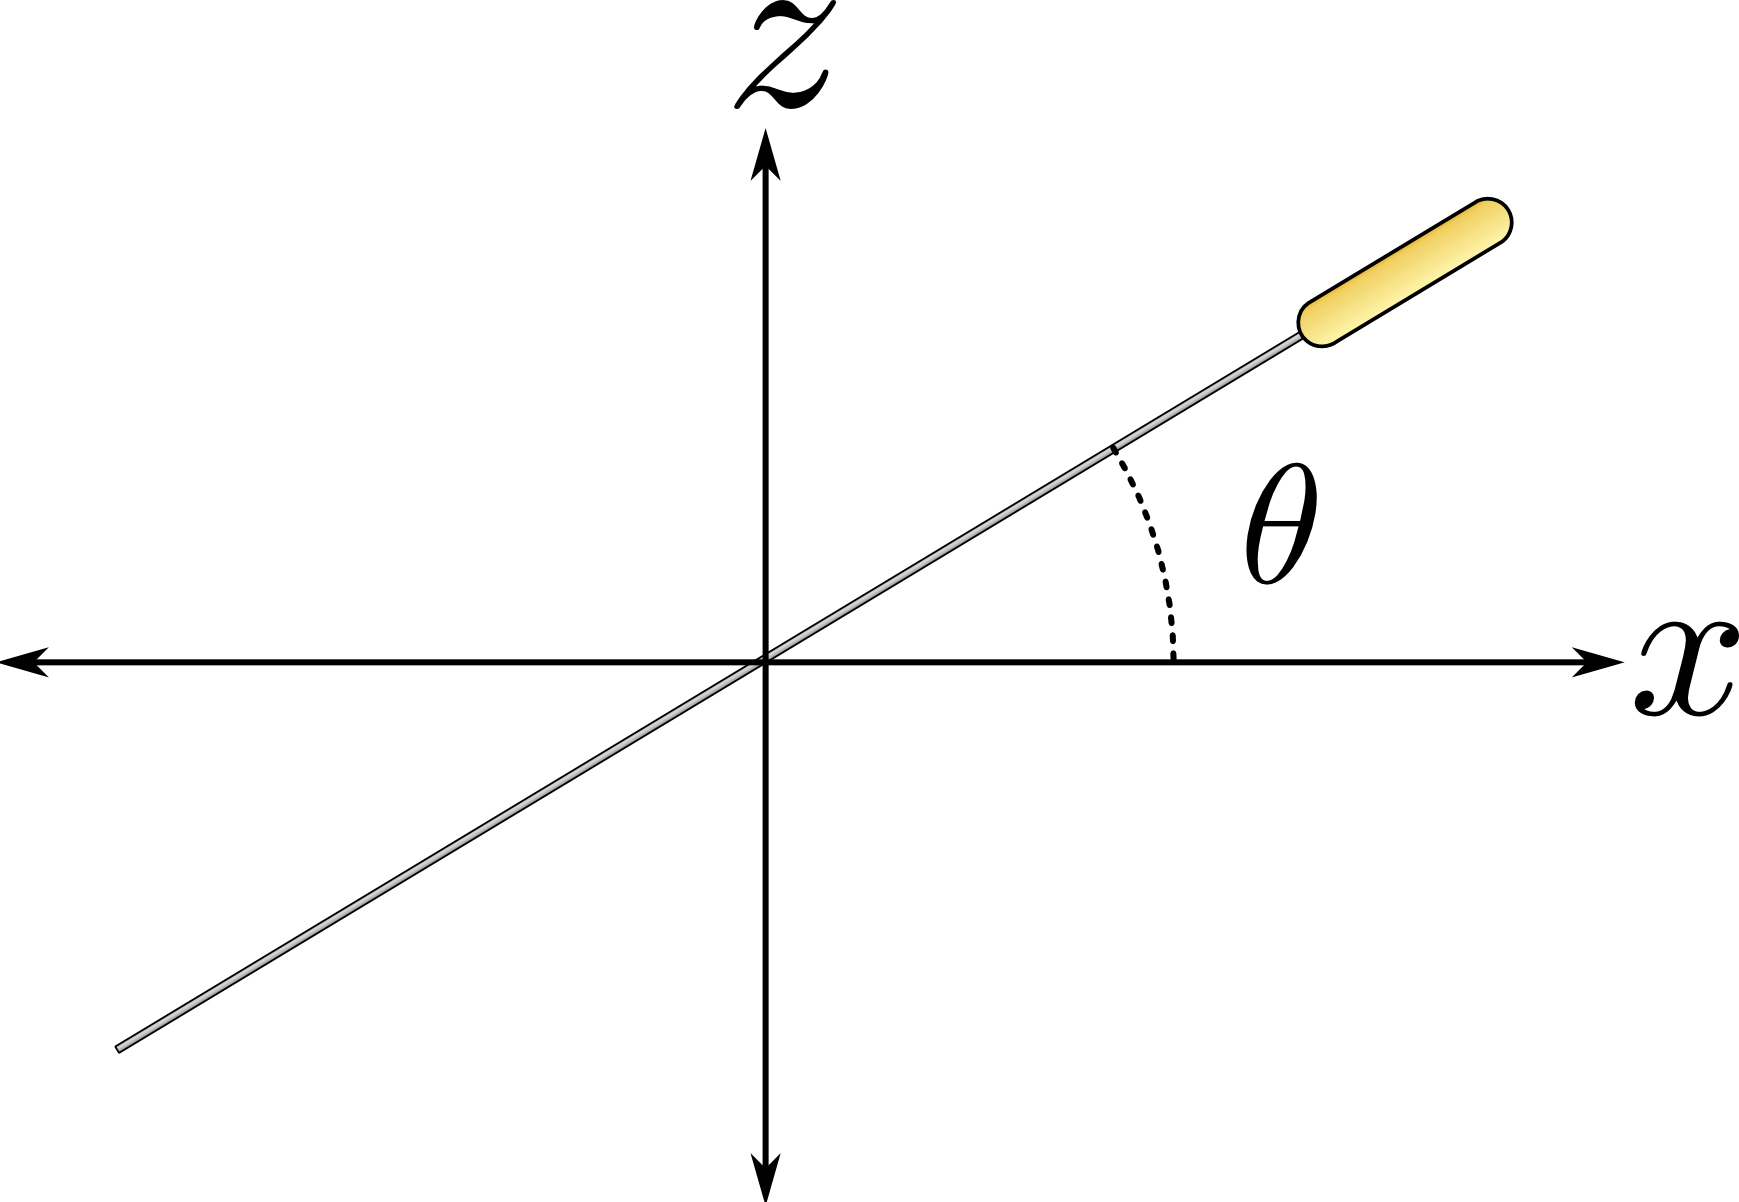
\includegraphics[width=0.3\textwidth]{fig/angle.png}
\label{fig:angle}
\caption{A diagram illustrating the measurement of angle in models and
measurements in this document. In all these cases, the angle is measured from
the horizontal plane, which is also the plane of isotropy. }
\end{figure}


\section{Document Outline}

First, this document will discuss the differential equations associated with
adapting the isotropic needle probe technique to the anisotropic case, as well
as analytical approaches to solving them. 

Second, the use of 3D finite element models in COMSOL with MATLAB to find 
numerical solutions to the problem will be discussed.

Then, this document will cover techniques for testing the predictions of the
these approaches with both real snow and engineered anisotropic materials, in
this case using table salt and table sugar.

The results of the analytical and numerical approaches will then be compared to
each other and the measurements of snow and engineered materials. The meanings
of these results are also discussed.

Finally, ``loose ends,'' unanswered questions, and avenues for future research
will be elucidated.

\chapter{Analytical Needle Probe Approach}
\label{sec:analytical-np}
\bigskip

\section{Introduction}

The technique used to measure thermal conductivity with a needle probe is based
on the assumption that the needle approximates an infinite line source of energy
with a constant heat flux embedded in an infinite medium. The origins of the
analytical solution for isotropic thermal conductivity may be found in Carslaw
and Jaeger's book, ``Conduction of Heat in Solids.'' \cite{basictheory}

The method based on Carslaw and Jaeger's solution depends on solving a 2-D
problem, where all planes orthogonal to the needle have the same temperature
distribution; in other words, temperature is not a function of axial position.
Moreover, the problem is further simplified by posing the problem into radial
coordinates and solving for temperature as a function of radial distance only.

In the isotropic case, this is straightforward, as conductivity is a constant
scalar. Unfortunately the anisotropic case is more complex, but luckily not
completely intractible.

\section{The Isotropic Case}

The isotropic case solves the following equation:

\begin{equation*}
k\nabla^2 T = \rho C\frac{\partial T}{\partial t}
\end{equation*}

Where \(T\) is temperature, \(k\) is a scalar thermal conductivity, \(\rho\) is
density, \(C\) is volumetric heat capacity, and \(t\) is time.

By casting this problem into cylindrical coordinates, the equations may be
simplified such that they are a function of radial distance \(r\) only (as
temperature is assumed to not be a function of axial position \(z\) or angle
\(\phi\)).

After applying this transformation and solving the equation, the analytical
solution to the problem becomes:

\begin{equation}
\label{isotropic_ei}
T(r,t) = - \frac{q}{4\pi k}\Ei\left(-\frac{r^2}{4kt}\right)
\end{equation}

where \(q\) is heat flux from the needle per linear distance, and \(\Ei()\) is
as defined in Equation \ref{eq:ei} for real-valued arguments.

\begin{equation}
\label{eq:ei}
\Ei(x) = -\int_{-x}^{\infty} \frac{e^{-t}}{t}dt
\end{equation}

Solving for the exponential integral analytically is not possible, and numerical
solutions can be difficult. Typically, an approximation for small
\(r^2/t\) is used instead:

\begin{equation}
\label{isotropic_case}
T(r,t) = \frac{q}{4\pi k}\ln\left(\frac{4kt}{r^2}\right) - \frac{\gamma q}{4\pi k}
\end{equation}

Typical use of this function is to find \(\frac{dT}{d(\ln t)}\) and solve
for \(k\). Equation \ref{isotropic_case} will be used for the remainder of
this analysis, though it could easily be applied to Equation \ref{isotropic_ei} as well.


\section{Difficulties in the Anisotropic Case}
\label{sec:analytical-np:anisotropic-diff}


The anisotropic case varies from the isotropic one in that instead of a scalar 
thermal conductivity \(k\), one must solve the problem using an \(n \times n\)
thermal conductivity, \([K]\), where \(n\) is the number of dimensions in the
problem. As a consequence, reducing the problem into two dimensions becomes more
difficult. Moreover, when the problem is posed in cylindrical coordinates, the
solution becomes a function not only of \(r\), but of \(\phi\) as well.

\section{Posing The Problem in Two Coordinates}
\label{sec:analytical-np:2D}

By assuming that temperature distribution is not a function of axial direction
\(z\), one may reduce the problem to an analogous one in orthogonal directions
\(x\) and \(y\) instead:

\begin{equation}
\nabla_{xy} \cdot \left([K]_{2 \times 2}\nabla_{xy} T \right)= \rho C\frac{\partial T}{\partial t}
\end{equation}

Without loss of generality, it may be further simplified like so:

\begin{equation}
\nabla \cdot \left(\begin{bmatrix}k_x & 0\\ 0 & k_y\end{bmatrix}\nabla T \right)= \rho C\frac{\partial T}{\partial t}
\end{equation}

This may be done by choosing the directions \(x\) and \(y\) such that the
matrix is diagonal.

The values of \(k_x\) and \(k_y\) may be found by finding the components of
\([K]\) that are in the \(xy\) plane.

%, as illustrated in \ref{fig:projection}. 
In particular, Equation \ref{eq:projection} was used in practice.

\begin{equation}
\label{eq:projection}
\left[ k_x, k_y \right] = 
\Eig\left(\begin{bmatrix} 1 & 0 & 0 \\ 0 & 1 & 0\\ 0 & 0 & 0\end{bmatrix}
\left[K\right]\right)
\end{equation}

\begin{comment}
\begin{figure}[h]
\centering
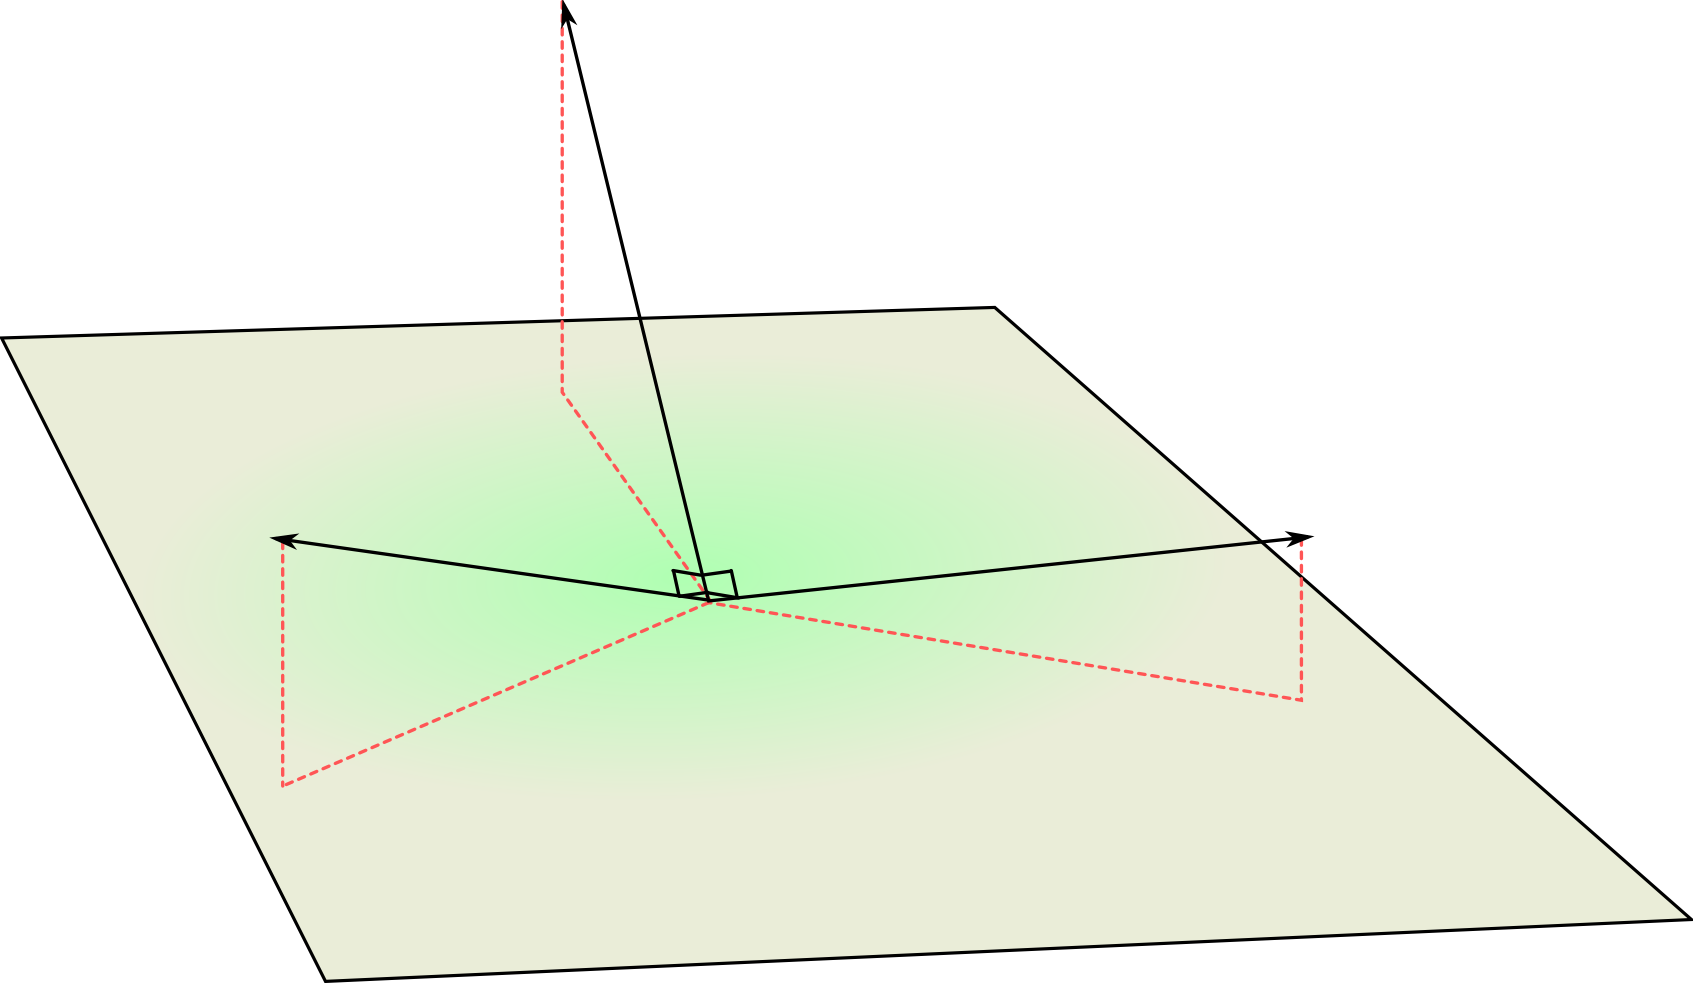
\includegraphics[width=0.6\textwidth]{fig/projection.png}
\label{fig:projection}
\caption{An informal demonstration of how the 3-D problem may be projected onto a 2-D domain.}
\end{figure}
\end{comment}

\section{Coordinate Transformation}
\label{sec:analytical-np:transformation}

\begin{figure}[h]
\centering
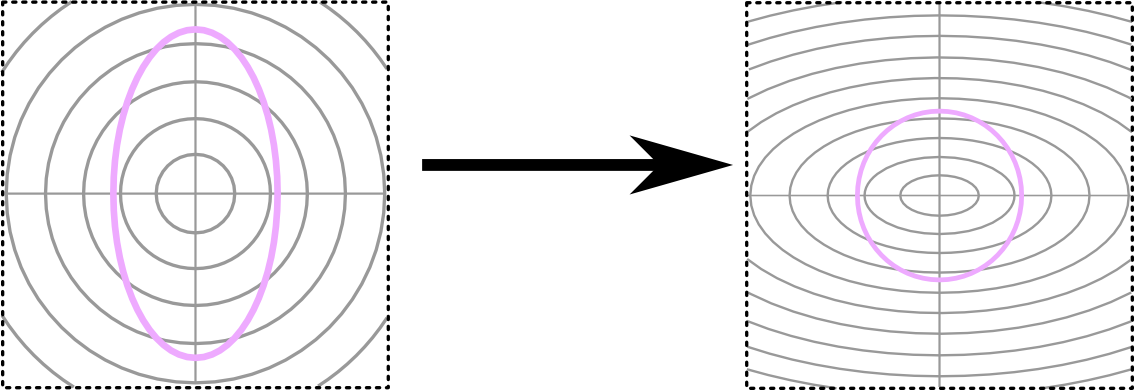
\includegraphics[width=0.8\textwidth]{fig/coordinate_transformation.png}
\caption{A 2-dimensional linear coordinate transformation.}
\label{fig:coord_trans}
\end{figure}

In order to apply the isotropic solution to this anisotropic case, a coordinate transformation may be applied such that the problem is transformed into
an isotropic case with respect to some \(x' = a_x x\) and \(y' = a_y y\), as in
Figure \ref{fig:coord_trans}.
Without loss of generality, suppose \(a_x = 1\).

\begin{align}
\frac{dx'}{dx} &= 1\\
\frac{dy'}{dy} &= a_y\\
\frac{\partial f}{\partial x} &= \frac{\partial f}{\partial x'}\frac{dx'}{dx} = \frac{\partial f}{\partial x'}\\
\frac{\partial f}{\partial y} &= \frac{\partial f}{\partial y'}\frac{dy'}{dy} = a_y\frac{\partial f}{\partial y'}\\
\nabla T &= \frac{\partial T}{\partial x'} \e_{x'} + a_y\frac{\partial T}{\partial y'} \e_{y'} \\
[K]\nabla T &= k_x\frac{\partial T}{\partial x'} \e_{x'} + k_ya_y\frac{\partial T}{\partial y'} \e_{y'}\\
\nabla \cdot \left([K]\nabla T\right) &= k_x\frac{\partial^2 T}{\partial {x'}^2} + k_ya_y^2\frac{\partial^2 T}{\partial {y'}^2}\\
\end{align}

Suppose the right hand side is equal to the equivalent isotropic expression:
\begin{equation}
k\left(\frac{\partial^2 T}{\partial {x'}^2} + \frac{\partial^2 T}{\partial {y'}^2} \right) = k_x\frac{\partial^2 T}{\partial {x'}^2} + k_ya_y^2\frac{\partial^2 T}{\partial {y'}^2}
\end{equation}

As a result,

\begin{align}
k &= k_x\\ a_y &= \sqrt{\frac{k_x}{k_y}}\\
\end{align}

Therefore, the following coordinate transformation will allow for the application
of isotropic solutions to an isotropic case with \(k = k_x\):

\begin{equation}
    \label{coord_trans}
    \begin{pmatrix}x' \\ y'\end{pmatrix} =
    \begin{bmatrix}1 & 0\\ 0 & \sqrt{\frac{k_x}{k_y}} \end{bmatrix}\begin{pmatrix}x \\ y\end{pmatrix}
\end{equation}

\section{From Temperature Distribution to Effective Thermal Conductivity}

Using Equation \ref{coord_trans}, the isotropic solution may be applied:

\begin{equation}
    k_x \nabla^2 T = \rho C\frac{\partial T}{\partial t}
\end{equation}

to yield the following result (for sufficiently large \(t/(r')^2\)):

\begin{equation}
T(r',t) = \frac{q}{4\pi k_x}\ln\left(\frac{4k_xt}{r'^2}\right) - \frac{\gamma q}{4\pi k_x}
\end{equation}

In the isotropic case, the value of \(r\) does not change the derivative with
respect to the natural log of time, as long as it is assumed constant. In contrast, the anisotropic case requires that another transformation is applied
to \(r'\) so that both \(k_x\) and \(k_y\) may be recovered. This requires that
some contextual meaning is assigned to \(r\) and \(r'\). In this analysis, it
is assumed that the measurement occurs at some  \(r = r_{\textrm{0}}\), perhaps
on the surface of the physical needle.

This approach isn't without its problems. For example, it supposes that the
isotherms are all circles in the transformed geometry, but if a finite-sized
needle was actually being modeled in the problem then the isotherms near the
(elliptically-shaped in the transformed domain) needle would be elliptical as
well, and only isotherms sufficiently far away would be round. However, this
approach allows us to keep using the \(\ln()\) approximation, while a solution
given a finite needle would likely require the use of Bessel functions.

Applying this technique to the anisotropic case, \(r_{xy} = \cos(\theta) \hat{e}_x + \sin(\theta) \hat{e}_y \) must also be transformed
into \(r_{x'y'}\):

\begin{align*}
    \begin{pmatrix}r_{x'} \\ r_{y'}\end{pmatrix} &=
    \begin{bmatrix}1 & 0\\ 0 & \sqrt{\frac{k_x}{k_y}} \end{bmatrix}\begin{pmatrix}r_0\cos(\theta) \\ r_0\sin(\theta)\end{pmatrix}\\
    &= r_0\left(\cos(\theta) \e_x + \sqrt{\frac{k_x}{k_y}} \e_y \right)\\
\end{align*}
\begin{equation}
    \norm{r'}^2 = r_0^2 \left(\cos^2(\theta) + \frac{k_x}{k_y}\sin^2(\theta) \right)\\
\end{equation}

This means that the temperature around the needle should now vary as a function
of \(\theta\), unlike in the isotropic case. Now, since the needle only measures
a single value, it may be assumed that the measured quantity is an
average temperature, such as the average surface temperature of the probe.  This
may be expressed like so:

\begin{equation}
\label{eq:tavg}
T_{\textrm{avg}}(t) = \frac{4\pi k_x}{q} \frac{\mathcal{E}(\ln(t), \frac{k_x}{k_y})}{\mathcal{E}(1, \frac{k_x}{k_y})}
\end{equation}

\hspace{-\parindent}where:

\begin{equation}
\mathcal{E}(f(\phi, \alpha), \alpha) = \int_0^{2\pi} f\sqrt{\cos^2(\phi) + \alpha\sin^2(\phi)} d\phi
\end{equation}

\section{Finding Effective Conductivity as a Function of Needle Orientation}

In order to extract the effective \(k\) value, a function of the form
\(C_1 \ln(t) + C_2\) is fit to Equation \ref{eq:tavg}. Then, all that is left is to evaluate the functions at various combinations of
\(k_xy\), \(k_z\) and \(\theta\).

\section{Conclusions}
\label{sec:analytical-np:conclusion}

An analytical approach to studying anisotropic thermal conductivity with needle
probes is more difficult than with the isotropic case. However, by using
coordinate projections to pose the problem in two dimensions, and by applying
coordinate transformations to the domain, one may apply the accepted isotropic
theory to the anisotropic case with minimal modification.  By numerically
evaluating the predicted temperature distribution over time, one may find the
expected conductivity measurement given the theory holds for anisotropic
materials.


\chapter{Numerical Needle Probe Approach}
\label{sec:numerical-np}
\bigskip

\section{Introduction} 
\label{sec:numerical-np:introduction}

Numerical experiments simulated needle probes in anisotropic mediums with
three-dimensional finite element heat transfer models in COMSOL 3.5a. While the
models themselves were relatively simple, attempting to automate a parameter
study in COMSOL 3.5a with respect to the anisotropic material properties proved
difficult.

\section{Geometry and Domain Properties}
\label{sec:numerical-np:domain}

\begin{table}[h]
\label{tab:constants}
\centering
\caption{Constants Used in Numerical Models}
\begin{tabular}{r | l}
radius of needle & \(0.25\) mm\\
length of needle & \(10\) cm\\
radius of snow & \(40\) cm\\
\hline
density of needle & \(8000\) kg/\(\textrm{m}^3\)\\
\(C_P\) of needle & \(460\) \textbf{*units*}\\
\(q\) of needle & \(0.5\) W/m\\
\(k\) of needle & \(160\) \textbf{*units*}\\
\hline
density of snow & \(200\) kg/\(\textrm{m}^3\)\\
\(C_P\) of snow & \(2050\) \textbf{*units*}
\end{tabular}
\end{table}

The needle was simulated as a long, thin steel cylinder embedded in the center
of a sphere of snow. While most of the dimensions and material properties were
held constant (see Table \ref{tab:constants}), the anisotropic conductivity of
the snow was parameterized in the form of a \(3\times3\) symmetric, positive
definite matrix.  In practice, this was done by specifying a diagonal matrix
\(\Lambda\) with positive eigenvalues \(k_{xy}\) and \(k_z\) and a rotation
matrix \(R\) around the \(x\) axis, and then defining \(K = R^T\Lambda R\) as in
equation \ref{eq:rotdiagrot} :

\begin{equation}
\label{eq:rotdiagrot}
K = \begin{bmatrix}
\cos(\theta) & 0 & \sin(\theta)\\
0 & 1 & 0\\
-\sin(\theta) & 0 &\cos(\theta)
\end{bmatrix}
\begin{bmatrix}
k_{xy} & 0 & 0\\
0 & k_{xy} & 0\\
0 & 0 & k_z
\end{bmatrix}
\begin{bmatrix}
\cos(\theta) & 0 & \sin(\theta)\\
0 & 1 & 0\\
-\sin(\theta) & 0 &\cos(\theta)
\end{bmatrix}
\end{equation}

The boundary conditions on the surface of the sphere enforced zero heat flux,
and the radius of the sphere was chosen such that the sphere approximated an
infinite medium.

Point temperatures recorded were the center of the needle, which corresponds to
the location of the thermocouple used in real-world experiments, and six points
on the surface of the snow, to ensure that the sphere was sufficiently large.

\section{MATLAB in Geometry-Based Parameter Studies Using COMSOL 3.5a}
\label{sec:numerical-np:matlab}

Unfortunately, COMSOL 3.5a did not have the facilities necessary to implement a
geometry-changing multi-parameter study as required from the GUI alone. However,
COMSOL 3.5a did have facilities for scripting with MATLAB. Unfortunately, I
found the facility to be poorly-documented, and, at least with the particular
install hosted by ARSC, buggy and prone to crashing.

MATLAB code written to implement the parameter study was largely auto-generated
by COMSOL, by building a base model in COMSOL 3.5a and exporting to an m-file.
This code was then split into two parts: The meshing code, and the solving code.
These pieces of code were wrapped in functions, called ``mesher'' and ``solver''
respectively, and used by a main procedure called ``worker.m.'' Contained in
``worker.m'' is a MATLAB structure with the constants outlined in section
\ref{sec:numerical-np:domain} called ``params'':

\small
\begin{minted}{matlab}
    params=struct('rsnow', 0.4, ...
                  'rneedle', 0.00025, ...
                  'lneedle', 0.1, ...
                  'density_snow', 200, ...
                  'density_needle', 8000, ...
                  'cp_snow', 2050, ...
                  'cp_needle', 460, ...
                  'q_needle', 0.5, ...
                  'k_needle', 160, ...
                  'time', [logspace(0.1,1,15) logspace(1,3,15)], ...
                  'angles', angles );
\end{minted}
\normalsize

This structure also contains a list of angles yet to be solved for, and the
times for which to solve.

The meshing code was wrapped in a function called ``mesher'' and took an angle
(in degrees) and the params structure as arguments, and is for the most part
simply code generated by COMSOL:

%% MESHER %%%%%%%%%%%%%%%%%%%%%%%%%%%%%%%%%%%%%
\small
\begin{minted}{matlab}

% COMSOL Multiphysics Model M-file
% Generated in part by COMSOL 3.5a (COMSOL 3.5.0.608, $Date: 2009/05/11 07:38:49 $)
% the rest of it modified by Joshua Holbrook

function fem=mesher(angle,params)
    % mesh_generate(angle)
    % generates a mesh for the given angle. 

    fprintf(['meshing for angle=' num2str(angle) '...\n']);

    flclear fem

    % COMSOL version
    clear vrsn
    vrsn.name = 'COMSOL 3.5';
    vrsn.ext = 'a';
    vrsn.major = 0;
    vrsn.build = 608;
    vrsn.rcs = '$Name: v35ap $';
    vrsn.date = '$Date: 2009/05/11 07:38:49 $';
    fem.version = vrsn;
\end{minted}
\normalsize

The COMSOL code was changed to use the arguments passed to ``mesher'' instead of
the values used in the original model:

\small
\begin{minted}{matlab}
    % Geometry
    g1=sphere3(num2str(params.rsnow),'pos',{'0','0','0'},'axis',{'0','0','1'},'rot','0');
    g2=cylinder3(num2str(params.rneedle),num2str(params.lneedle),'pos',{num2str(-params.lneedle/2),'0','0'},'axis',{'1','0','0'},'rot','0');
    parr={point3(0,0,0)};
    g3=geomcoerce('point',parr);
    parr={point3(params.rsnow,0,0)};
    g4=geomcoerce('point',parr);
    parr={point3(0,params.rsnow,0)};
    g5=geomcoerce('point',parr);
    parr={point3(0,0,params.rsnow)};
    g6=geomcoerce('point',parr);
    parr={point3(-params.rsnow,0,0)};
    g7=geomcoerce('point',parr);
    parr={point3(0,-params.rsnow,0)};
    g8=geomcoerce('point',parr);
    parr={point3(0,0,-params.rsnow)};
    g9=geomcoerce('point',parr);
\end{minted}
\normalsize

Here, it can be seen that a number of points are generated: First, the point
representing the thermocouple temperature at \((0, 0, 0)\), and then six points
over the surface of the sphere.

Notice that, in this code, ``theta'' is never actually used. This is
because, in early iterations of the code, the needle was rotated by the angle
``theta.'' However, this seemed to cause random errors from COMSOL's meshing
procedures, so the anisotropic thermal properties of the snow were changed
instead, as outlined in section \ref{sec:numerical-np:domain}. However, the
argument was retained in order to avoid editing other legacy code in the model.

Afterwards, geometry is labelled and a mesh is initialized and refined using
code generated by COMSOL, and returns the COMSOL ``fem'' structure:

\small
\begin{minted}{matlab}

    % Analyzed Geometry
    clear p s
    p.objs={g3,g4,g5,g6,g7,g8,g9};
    p.name={'ORIGIN','PT1','PT2','PT3','PT4','PT5','PT6'};
    p.tags={'g3','g4','g5','g6','g7','g8','g9'};

    s.objs={g1,g2};
    s.name={'SNOW','NEEDLE'};
    s.tags={'g1','g2'};

    fem.draw=struct('p',p,'s',s);
    fem.geom=geomcsg(fem);


    % ODE Settings
    clear ode
    clear units;
    units.basesystem = 'SI';
    ode.units = units;
    fem.ode=ode;


    % Initialize mesh
    fem.mesh=meshinit(fem, ...
                      'hauto',5, ...
                      'hgradsub',[2,1.1], ...
                      'hmaxsub',[2,0.0005]);

    % Refine mesh
    fem.mesh=meshrefine(fem, ...
                        'mcase',0, ...
                        'rmethod','longest');

    fem=multiphysics(fem);
end
\end{minted}
\normalsize

This ``fem'' structure may then be passed to the ``solver'' function, along
with parameters describing the snow's material properties and the needle's
orientation with respect to the snow. Similarly, the ``solver'' function is
mostly COMSOL code wrapped in a function:

\small
\begin{minted}{matlab}
% COMSOL Multiphysics Model M-file
% Generated by COMSOL 3.5a (COMSOL 3.5.0.608, $Date: 2009/05/11 07:38:49 $)
% the rest of it modified by Joshua Holbrook

function answer=solver(kxy,kz,fem,theta,params)
    %solver(kxy,kz,mesh,theta,params)
    %uses comsol to pump out a solution using a given mesh-mat and a k-matrix in comsol format.

    fprintf(['solving for kxy=' num2str(kxy) ' and kz=' num2str(kz) '...\n']);
    % Application mode 1
    clear appl
    appl.mode.class = 'GeneralHeat';
    appl.module = 'HT';
    appl.shape = {'shlag(1,''J'')','shlag(2,''T'')'};
    appl.sshape = 2;
    appl.assignsuffix = '_htgh';
    clear bnd
    bnd.type = {'q0','cont'};
    bnd.shape = 1;
    bnd.ind = [1,1,1,1,2,2,2,2,2,1,1,1,1,2];
    appl.bnd = bnd;
    clear equ
    equ.sdtype = 'gls';
\end{minted}
\normalsize

Here, parameters or the material properties are attached to the domain:

\small
\begin{minted}{matlab}
    % densities
    equ.rho = {params.density_snow,params.density_needle};
    equ.init = 0;
    equ.shape = 2;
    % Heat capacities
    equ.C = {params.cp_snow,params.cp_needle};
    % Wattage
    equ.Q = {0,params.q_needle/pi/(params.rneedle)^2};
    % Heat conductivities
    arr = [cos(theta*pi/180), 0, sin(theta*pi/180); 0, 1, 0; -sin(theta*pi/180), 0, cos(theta*pi/180)]; %rotation matrix
    equ.k = {symmetric_tocell(arr*diag([kxy,kxy,kz])*(arr')),params.k_needle};
\end{minted}
\normalsize

This is also where the symmetric matrix is generated, as described in section
\ref{sec:numerical-np:domain}. ``symmetric\_tocell'' is a helper function which
converts symmetric matrices of the form 
\minted{matlab}{[a1 a2 a4; a2 a3 a5; a4 a5 a6]} to the form
\minted{matlab}{ {a1, a2, a3, a4, a5, a6 }}.

Then, more code generated by COMSOL:

\small
\begin{minted}{matlab}
    equ.ind = [1,2];
    appl.equ = equ;
    fem.appl{1} = appl;
    fem.frame = {'ref'};
    fem.border = 1;
    fem.outform = 'general';
    clear units;
    units.basesystem = 'SI';
    fem.units = units;

    % Coupling variable elements
    clear elemcpl
    % Integration coupling variables
    clear elem
    elem.elem = 'elcplscalar';
    elem.g = {'1'};
    src = cell(1,1);
    clear bnd
    bnd.expr = {{'T',{}},{'1',{}}};
    bnd.ipoints = {{'4',{}},{'4',{}}};
    bnd.frame = {{'ref',{}},{'ref',{}}};
    bnd.ind = {{'1','2','3','4','10','11','12','13'},{'5','6','7','8','9', ...
      '14'}};
    src{1} = {{},{},bnd,{}};
    elem.src = src;
    geomdim = cell(1,1);
    geomdim{1} = {};
    elem.geomdim = geomdim;
    elem.var = {'int_T','area'};
    elem.global = {'1','2'};
    elemcpl{1} = elem;
    fem.elemcpl = elemcpl;

    % ODE Settings
    clear ode
    clear units;
    units.basesystem = 'SI';
    ode.units = units;
    fem.ode=ode;

    % Multiphysics
    fem=multiphysics(fem);

    % Generate GMG mesh cases
    fem=meshcaseadd(fem,'mgauto','anyshape');

    % Extend mesh
    fem.xmesh=meshextend(fem);

    % Solve problem
    fem.sol=femtime(fem, ...
                    'solcomp',{'T'}, ...
                    'outcomp',{'T'}, ...
                    'blocksize','auto', ...
                    'tlist', params.time, ...
                    'estrat',1, ...
                    'tout','tlist', ...
                    'linsolver','gmres', ...
                    'itrestart',100, ...
                    'prefuntype','right', ...
                    'prefun','gmg', ...
                    'prepar',{'presmooth','ssor','presmoothpar',{'iter',3,'relax',0.8},'postsmooth','ssor','postsmoothpar',{'iter',3,'relax',0.8},'csolver','pardiso'}, ...
                    'stopcond','0.06-int_T/area', ...
                    'mcase',[0 1]);

    % Save current fem structure for restart purposes
    fem0=fem;
\end{minted}
\normalsize

Code to plot the solution was commented out and replaced with code to save the
temperature data at the center of the needle, and the average temperature of the
six points at the surface of the sphere, to MATLAB variables:

\small
\begin{minted}{matlab}

    % Plot solution
    %{
    postplot(fem, ...
             'slicedata',{'T','cont','internal','unit','K'}, ...
             'slicexspacing',5, ...
             'sliceyspacing',0, ...
             'slicezspacing',0, ...
             'slicemap','Rainbow', ...
             'solnum','end', ...
             'title','Time=100    Slice: Temperature [K]', ...
             'grid','on', ...
             'campos',[-2.636014311828346,-3.4353207343472505,2.4999999999999996], ...
             'camtarget',[0,0,0], ...
             'camup',[0,0,1], ...
             'camva',41.213465344831754);
    %}

    % Integrate
    T_thermistor=postint(fem,'T', ...
               'unit','K', ...
               'recover','off', ...
               'dl',8, ...
               'edim',0, ...
               'solnum','all');

    % Integrate
    T_surf_avg=postint(fem,'T', ...
               'unit','', ...
               'recover','off', ...
               'dl',[1,2,3,4,10,11,12,13], ...
               'edim',2, ...
               'solnum','end');
\end{minted}
\normalsize

Finally, the data is packed into a cell array, and the ``angles'' parameter
is changed:

\small
\begin{minted}{matlab}

    answer={[fem.sol.tlist; T_thermistor],T_surf_avg};
    angles = params.angles(2:length(params.angles));

    %flsave(['fem-' num2str(theta) '-' num2str(kxy) '-' num2str(kz) '.mph']);

    save('angles.m', 'angles');
end
\end{minted}
\normalsize

In some runs, the fem structure was exported back to the COMSOL format for
further study.

\section{Automatic Calculation of Conductivity from Simulated Time/Temperature Data}

Results from COMSOL were automatically fitted against the linear model with
respect to \(\ln(t)\) by ``dropping'' early \((t,T)\) datapoints until the
correlation coefficient of the remaining points was sufficiently high. Then, a
linear curvefit was applied to these remaining points. Finally, the slope was
used to calculate \(k_{\textrm{meas}}\).

\small
\begin{minted}{matlab}
function k = fitter(t,T,rset,params)
    logt = log(t(t>1));
    T = T(t>1);

    disp('Finding linear portion...');    
    for i=1:length(logt)-1
        C = corrcoef(logt(i:length(logt)), T(i:length(T)));
        r = sqrt(C(2,1));
        if r > rset %adjust this to get 'good' values
            disp([ 'linear fitting to ' ...
                   num2str((length(logt)-i)) ...
                   ' points from t=' num2str(exp(logt(i))) ...
                   ' to t=' ...
                   num2str(exp(logt(length(logt)))) ...
                   '...']);
            x = polyfit(logt(i:length(logt)),T(i:length(T)), 1);
            break
        end
    end

    k = (params.q_needle)/(4*pi*x(1));
end
\end{minted}
\normalsize

\section{Organization and Serialization of Results}

Simulation results were saved in a .mat file, which is MATLAB's native
serialization format. Results were organized into a nested cell array which
mirrored the format of two MATLAB matrices k\_xy and k\_z:

These functions were called by ``worker.m,'' which was used to run multiple
tests and save the results.

%% WORKER %%%%%%%%%%%%%%%%%%%%%%%%%%%%%%%%%%%%%
\small
\begin{minted}{matlab}
%worker.m
%does the working

function worker(kxy,kz)
    load('angles.mat', 'angles');
    angles
    [kxy,kz] = meshgrid(kxy,kz);

    %flreport('off');

    params=struct('rsnow', 0.4, ...
                  'rneedle', 0.00025, ...
                  'lneedle', 0.1, ...
                  'density_snow', 200, ...
                  'density_needle', 8000, ...
                  'cp_snow', 2050, ...
                  'cp_needle', 460, ...
                  'q_needle', 0.5, ...
                  'k_needle', 160, ...
                  'time', [logspace(0.1,1,15) logspace(1,3,15)], ...
                  'angles', angles );

    saveroot=['./solutions-' date '/'];

    mesh = mesher(0,params);
    for angle=angles,
        try
            solutions = arrayfun(@(x,y) solver(x,y,mesh,angle,params), ...
                            kxy,kz, 'UniformOutput', false);
            save solutions
            fprintf('Fitting solutions...\n');
            solutions = {cellfun(@(tsd) {fitter(tsd{1}(1,:),tsd{1}(2,:), ...
                                             0.999,params), ...
                             tsd{1}, tsd{2}}, ...
                         solutions, 'UniformOutput', false)};
            fprintf('A solution set just completed.');
            system([ 'echo "A solution set finished on" `hostname` ' ...
                     '| mutt -s "A solution set completed." ' ...
                     'josh.holbrook@gmail.com' ]);
        catch exception
            system([ 'echo "Exception occurred on" `hostname` ' ...
                     '| mutt -s "Exception occurred--' exception.message ...
                     '" josh.holbrook@gmail.com' ]);
        end
        angles = angles(2:length(angles));
        save('angles.mat', 'angles');
        %solutions
        mkdir(saveroot);
        save([ saveroot 'solution-' num2str(angle) ], ...
             'solutions','angle','kxy','kz','params');
    end

    % Emails me when everything's done
    system([ 'echo "Results completed on " `hostname` ' ...
             '| mutt -s "Results Completed" ' ...
             'josh.holbrook@gmail.com' ]);
    system('touch down');
end
\end{minted}
\normalsize
%%%%%%%%%%%%%%%%%%%%%%%%%%%%%%%%%%%%%

The data stored in each slot of the nested array was itself a cell array
containing the simulation results, as shown in figure \ref{fig:cellarray}:

% Bastardization of tabular use.
\begin{figure}
\label{fig:cellarray}

\centering
\begin{tabular}{| c | c | c |}
\hline
\(k_\textrm{meas}\) & \( \left[ \textrm{time}, \textrm{temperature} \right]^T\) & Average surface temperature of sphere\\
\hline
\end{tabular}
\caption{Contents of the cell array.}
\end{figure}

\section{Post-Simulation Analysis with MATLAB}

\section{Code Architecture and Use}

% \section{Verification with Analytical Approach}

\include{conclusions}

\appendix
\include{appendix_1}
\include{appendix_2}

\end{document}
